\subsection{آموزش مدل‌ها و خروجی}\label{subsec:آموزش مدل‌ها و خروجی}
برای فرآیند آموزش، مدل‌های معرفی شده در بخش قبل هرکدام به صورت جداگانه مورد و مستقل آموزش داده شدند. این مدل‌ها بر روی دو مجموع‌داده پاپسوسایتی و پایگاه داده ریزآرایه استنفورد و روش‌های مختلف داده افزایی مورد آزمایش قرار گرفتند. که در مجموع 1258 تصویر برای آموزش، 174 تصویر برای ارزیابی و 378 تصویر نیز برای تست به‌کار گرفته شد. نکته‌ای که در هنگام تقسیم بندی تصاویر به سه گروه آموزش، ارزیابی و تست باید در نظر گرفت، این است که نباید تصویری از یک اسلاید در دو گروه قرار بگیرند. به عنوان مثال، اگر از یک اسلاید چند تصویر استخراج شود باید تصاویر استفاده‌شده تنها در یکی از این سه گروه قرار بگیرند زیرا این تصاویر توزیع بسیار نزدیکی بهم دارند در نتیجه، قرار دادن آن‌ها در یک گروه به ارزیابی بهتر مدل کمک می‌کند.
نتایج نهایی اجراها در جدول \ref{table:papsociety_and_stanford_run_results} آمده است.
در ستون اول این جدول مدل‌های مورد آزمایش، در ستون دوم روش‌های داده افزایی مختلف، ستون سوم بهترین دور در حین فرآیند آموزش، ستون چهارم دقت نهایی در تشخیص بدخیم و یا خوشخیم بودن تصویر و ستون آخر نیز ویژگی عملکرد گیرنده\LTRfootnote{Receiver operating characteristic - ROC} برای گروه بدخیم آمده است. دقت به صورت میانگین دقت مدل در دو گروه محاسبه شده است.
روش‌های داده افزایی که در ستون دوم ذکر شده و به‌کار گرفته شد به چند گروه متفاوت دسته بندی می‌شوند. منظور از \lr{mixup} همان روش ادغام تصاویر است. منظور از \lr{fda} نیز روش تطبیق دامنه فوریه است و \lr{jit} نیز تغییر تصادفی رنگ تصویر است و در نهایت منظور از \lr{all} ترکیبی از هر سه روش است. در این ستون دو کلمه دیگر نیز دیده می‌شود. کمله \lr{base} اشاره به ترکیبی از روش‌های آیینه کردن، چرخاندن، تغییر مقیاس و اضافه کردن نویز گوسی دارد و کلمه \lr{base-nrs} تنها تفاوتی که در روش داده‌افزایی دارد عدم وجود روش تغییر مقیاس است. در نهایت \lr{none} اشاره به عدم استفاده از داده‌افزایی می‌کند.
\begin{table}[t]
	\centering
	\begin{latin}
		\begin{tabular}{|c|c|c|c|c|}
			\hline
			\rl{معماری شبکه} & \rl{روش‌های داده‌افزایی} & \rl{بهترین دور} & \rl{دقت} & \rl{مساحت زیر نمودار \lr{ROC}} \\
			\hline
			\hline
			\text{Inception V4} & \lr{none}            & $17$ & $92.94$ & $0.965$ \\
			\text{Inception V4} & \lr{base \& mixup}   & $85$ & $92.16$ & $0.967$ \\
			\text{Inception V4} & \lr{base \& fda}     & $85$ & $91.44$ & $0.944$ \\
			\text{Inception V4} & \lr{base \& jit}     & $58$ & $93.73$ & $0.976$ \\
			\text{Inception V4} & \lr{base \& all}     & $7$  & $93.88$ & $0.966$ \\
			\text{Inception V4} & \lr{base-nrs \& jit} & $9$  & $92.69$ & $0.944$ \\
			\text{Inception V4} & \lr{base-nrs \& all} & $27$ & $94.67$ & $0.943$ \\
			\hline
			\hline
			\text{Inception V3} & \lr{none}            & $56$ & $91.25$ & $0.937$ \\
			\text{Inception V3} & \lr{base \& mixup}   & $81$ & $93.63$ & $0.957$ \\
			\text{Inception V3} & \lr{base \& fda}     & $99$ & $93.73$ & $0.974$ \\
			\text{Inception V3} & \lr{base \& jit}     & $2$  & $91.34$ & $0.956$ \\
			\text{Inception V3} & \lr{base \& all}     & $75$ & $93.41$ & $0.966$ \\
			\text{Inception V3} & \lr{base-nrs \& jit} & $40$ & $92.06$ & $0.937$ \\
			\text{Inception V3} & \lr{base-nrs \& all} & $75$ & $93.41$ & $0.966$ \\
			\hline
			\hline
			\text{Resnet101}    & \lr{none}            & $14$ & $93.10$ & $0.971$ \\
			\text{Resnet101}    & \lr{base \& mixup}   & $84$ & $92.22$ & $0.951$ \\
			\text{Resnet101}    & \lr{base \& fda}     & $40$ & $94.04$ & $0.964$ \\
			\text{Resnet101}    & \lr{base \& jit}     & $99$ & $92.47$ & $0.947$ \\
			\text{Resnet101}    & \lr{base \& all}     & $25$ & $92.53$ & $0.962$ \\
			\text{Resnet101}    & \lr{base-nrs \& jit} & $55$ & $92.28$ & $0.925$ \\
			\text{Resnet101}    & \lr{base-nrs \& all} & $25$ & $92.53$ & $0.962$ \\
			\hline
			\hline
			\text{Resnet18}     & \lr{none}            & $55$ & $89.75$ & $0.922$ \\
			\text{Resnet18}     & \lr{base \& mixup}   & $7$  & $91.59$ & $0.934$ \\
			\text{Resnet18}     & \lr{base \& fda}     & $48$ & $94.51$ & $0.943$ \\
			\text{Resnet18}     & \lr{base \& jit}     & $94$ & $94.98$ & $0.974$ \\
			\text{Resnet18}     & \lr{base \& all}     & $80$ & $93.88$ & $0.962$ \\
			\text{Resnet18}     & \lr{base-nrs \& jit} & $90$ & $90.78$ & $0.939$ \\
			\text{Resnet18}     & \lr{base-nrs \& all} & $13$ & $94.10$ & $0.985$ \\
			\hline
		\end{tabular}
	\end{latin}
	\caption{نتایج آموزش  با مدل‌های مختلف و روش‌های داده افزایی متفاوت بر روی مجموع دو مجموع‌داده پاپسوسایتی و ریزآرایه بافت استنفورد}
	\label{table:papsociety_and_stanford_run_results}
\end{table}
در ادامه از مجموع‌داده اطلس ژنوم سرطان تیروئید برای آموزش مدل \lr{ResNet101} استفاده شد. همانطور که در فصل‌های پیش نیز اشاره شد، برچسب‌های این مجموع‌داده به صورت در صد سلول‌ها نرمال و توموری تهیه شده است. در ادامه سعی شده تا دسته بندی بر روی این مجموع‌داده آموزش داده شود تا با داشتن تصویر، وجود یا عدم وجود سلول‌های توموری را تشخیص دهد. تعداد تصاویری که در نهایت از این مجموع‌داده استخراج شد، 265418 است که از 185090 تصویر برای آموزش، 25909 تصویر برای ارزیابی و 54419 برای تست استفاده شد. باز باید روی این نکته تاکید کرد که تصاویر استخراج‌شده از یک اسلاید نباید در دو گروه قرار بگیرند.
با توجه به حجم زیاد داده‌ها و زمان بر بودن پردازش، در این قسمت تنها از روش \lr{mixup} و \lr{base} برای پیش‌پردازش استفاده شد. مدل در $20$ دور\LTRfootnote{Epoch} بر روی داده‌ها آموزش داده شد. دقت و نمودار‌های مربوط به آن در تصویر \ref{nci_dataset_with_resnet101_results} آمده است. دستگاه گرافیک به‌کار رفته مدل \lr{Quadro RTX 8000} بوده و زمان اجرا $32$ ساعت طول کشیده است.
\begin{figure}
	\begin{center}
		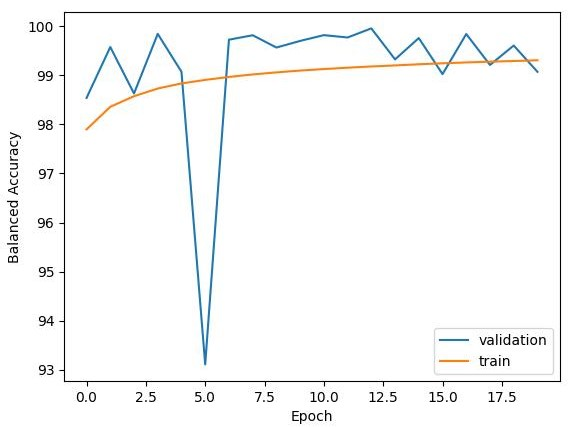
\includegraphics[width=0.8\linewidth]{figs/suggested_methods/val_train_acc_final.jpeg}
	\end{center}
	\caption[نمودار دقت در هر دوره آموزش]{بهترین دوره انتخاب شده دوره 12 بوده که دقت و ویژگی عملکرد گیرنده  بر روی داده‌های تست در این دوره به ترتیب $99.72$ و $0.9998$ است.}
	\label{nci_dataset_with_resnet101_results}
\end{figure}





